\documentclass[12pt]{article}
\usepackage{mathtext} 
\usepackage{amsmath}
\usepackage{multirow}
\usepackage{hhline}

\usepackage[english, russian]{babel}
\usepackage[TS1, T2A]{fontenc}
\usepackage[utf8]{inputenc}
\usepackage{pscyr}

\usepackage{fp}
\usepackage{xfp}
\usepackage{pgfplots}
\pgfplotsset{compat=1.9}


\usepackage{siunitx}
\sisetup{output-decimal-marker={,}}

\usepackage[left=2cm,right=2cm, top=1cm,bottom=1.5cm,bindingoffset=0cm]{geometry}

\usepackage{graphicx}
\graphicspath{{pictures/}}
\DeclareGraphicsExtensions{.pdf,.png,.jpg}

\begin{document}
	\pagestyle{empty}
	\begin{center}
		\normalsize
		\textbf{Федеральное государственное автономное образовательное учреждение высшего образования}

		\small
		\medskip 
		\textbf{САНКТ-ПЕТЕРБУРГСКИЙ НАЦИОНАЛЬНЫЙ ИССЛЕДОВАТЕЛЬСКИЙ  УНИВЕРСИТЕТ ИНФОРМАЦИОННЫХ ТЕХНОЛОГИЙ, МЕХАНИКИ И ОПТИКИ}

		\medskip 
		\textbf{ФАКУЛЬТЕТ ПРОГРАММНОЙ ИНЖЕНЕРИИ И КОМПЬЮТЕРНОЙ ТЕХНИКИ}	
	\bigskip\bigskip\bigskip\bigskip\bigskip\bigskip\bigskip\bigskip\bigskip\bigskip\bigskip\bigskip	
		\par\medskip\par\smallskip\par\smallskip
		\Large 
		\textbf{ОТЧЕТ} 

		\textbf{ПО ЛАБОРАТОРНОЙ РАБОТЕ №1}

		\large
		\par\bigskip
		\textbf{«Исследование характеристик источника электрической энергии постоянного тока»}
		\par\bigskip\par\bigskip\par\bigskip\par\bigskip\par\bigskip\par\bigskip
		\par\bigskip\par\bigskip\par\bigskip\par\bigskip\par\bigskip\par\bigskip
		\par\bigskip\par\bigskip\par\bigskip\par\bigskip\par\bigskip\par\bigskip
		\normalsize
		\begin{tabular}{lllll}
							\hspace{170pt}	 							& \hspace{80pt}	&	Выполнил:								&\\
																	&			&	Студент группы P3255					&\\
																	& 			&	Федюкович С. А. \_\_\_\_\_\_\_\_\_\_\_\_\_\_	&\\
																	&			&										&\\
																	&			&										&\\
		\end{tabular}
		\par\bigskip\par\bigskip\par\bigskip                                                  
		\par\bigskip \par\bigskip
		\par\bigskip\par\bigskip\par\bigskip\par\bigskip\par\bigskip\par\bigskip\par\bigskip\par\bigskip
		
		Санкт-Петербург
		\par\bigskip
		2018
	\end{center}
	\newpage
	\pagestyle{plain}
	\setcounter{page}{1}
	\section*{Цель работы}
	Исследование режимов работы и экспериментальное определение параметров схемы замещения источника электрической энергии.
	\section*{Ход работы}
	\begin{enumerate}
		\FPset{E}{240}
		\FPset{r}{3200}
		\item В приложении LTspice собрать электрическую цепь  по заданной схеме замещения со значениями $r=\num{\r}[Ом]$ и $E=\num{\E}[В]$(рис.1).
			\begin{figure}[h]
				\center{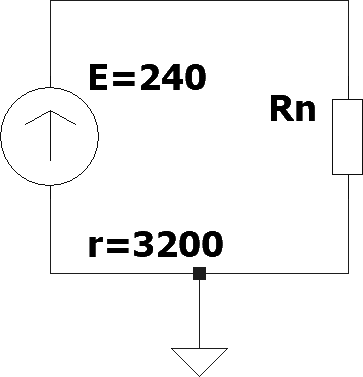
\includegraphics[scale=0.75]{1}}
				\caption{Схема электрической цепи}
				\label{fig:image}
			\end{figure}		
		
		\FPset{uZero}{\E}
		\item Измерить напряжение холостого хода $U_0$ при разрыве цепи, занести полученный результат в таблицу 1.		
		
		\FPset{rOne}{\r}
		\FPeval{\uOne}{round(uZero/2,3)}
		\item Изменяя сопротивление $R_n$ найти такое $R_n$,при котором $U_n = \frac{U_0}{2} = \frac{\num{\uZero}}{2}=\num{\uOne} [Ом]$. Занести в таблицу значение $R_n$.			
			
		\item Заполнить таблицу, изменяя сопротивление от $100[Ом]$ до $10000[Ом]$ соответствующими значениями $U_k$.
		\FPset{rTwo}	{10000.000}		\FPset{uTwo}	{181.818}		
		\FPset{rThree}	{8000.000}		\FPset{uThree}	{171.428}		
		\FPset{rFour}	{6000.000}		\FPset{uFour}	{156.521}	
		\FPset{rFive}	{5000.000}		\FPset{uFive}	{146.341}		
		\FPset{rSix}	{2500.000}		\FPset{uSix}	{105.263}		
		\FPset{rSeven}	{1000.000}		\FPset{uSeven}	{57.142}		
		\FPset{rEight}	{500.000}		\FPset{uEight}	{32.432}		
		\FPset{rNine}	{250.000}		\FPset{uNine}	{17.391}		
		\FPset{rTen}	{100.000}		\FPset{uTen}	{7.272}	
		
		\item Для каждого $k$ рассчитать ток в нагрузке по формуле $I_k = \frac{U_k}{R_k}$ [А]:
		\FPset{m}{1000.000}
		\FPset{iZero}{0.000}
		\FPeval{\iOne}		{round(uOne/rOne*m		,3)}
		\FPeval{\iTwo}		{round(uTwo/rTwo*m		,3)}
		\FPeval{\iThree}	{round(uThree/rThree*m	,3)}
		\FPeval{\iFour}		{round(uFour/rFour*m	,3)}
		\FPeval{\iFive}		{round(uFive/rFive*m	,3)}
		\FPeval{\iSix}		{round(uSix/rSix*m		,3)}
		\FPeval{\iSeven}	{round(uSeven/rSeven*m	,3)}
		\FPeval{\iEight}	{round(uEight/rEight*m	,3)}
		\FPeval{\iNine}		{round(uNine/rNine*m	,3)}
		\FPeval{\iTen}		{round(uTen/rTen*m		,3)}		
		\begin{table}[h!]
			\begin{center}
				\begin{tabular}{ll}
					$I_0 = \frac{U_0}{R_0} = \frac{\num{\uZero}}{\infty} \cdot \num{\m} \approx \num{\iZero} [мА];$ & $I_6 = \frac{U_6}{R_6} = \frac{\num{\uSix}}{\num{\rSix}} \cdot \num{\m} \approx \num{\iSix} [мА];$ \\
							
					$I_1 = \frac{U_1}{R_1} = \frac{\num{\uOne}}{\num{\rOne}} \cdot \num{\m} \approx \num{\iOne} [мА];$ & $I_7 = \frac{U_7}{R_7} = \frac{\num{\uSeven}}{\num{\rSeven}} \cdot \num{\m} \approx \num{\iSeven} [мА];$ \\ 
										
					$I_2 = \frac{U_2}{R_2} = \frac{\num{\uTwo}}{\num{\rTwo}} \cdot \num{\m} \approx \num{\iTwo} [мА];$ & $I_8 = \frac{U_8}{R_8} = \frac{\num{\uEight}}{\num{\rEight}} \cdot \num{\m} \approx \num{\iEight} [мА];$ \\
							
					$I_3 = \frac{U_3}{R_3} = \frac{\num{\uThree}}{\num{\rThree}} \cdot \num{\m} \approx \num{\iThree} [мА];$ & $I_9 = \frac{U_9}{R_9} = \frac{\num{\uNine}}{\num{\rNine}} \cdot \num{\m} \approx \num{\iNine} [мА];$ \\
							
					$I_4 = \frac{U_4}{R_4} = \frac{\num{\uFour}}{\num{\rFour}} \cdot \num{\m} \approx \num{\iFour} [мА];$ & $I_{10} = \frac{U_{10}}{R_{10}} = \frac{\num{\uTen}}{\num{\rTen}} \cdot \num{\m} \approx \num{\iTen} [мА];$ \\					
		
					$I_5 = \frac{U_5}{R_5} = \frac{\num{\uFive}}{\num{\rFive}} \cdot \num{\m} \approx \num{\iFive} [мА].$ &  \\	
				\end{tabular}
			\end{center}
		\end{table}
		
		\newpage
		\item Для каждого $k$ рассчитать рассеиваемую в нагрузке мощность по формуле $P_k = \frac{{U_k}^2 }{ R_k}$ [Вт] :
		\FPset{pZero}{0.000}
		\FPeval{\pOne}		{round(uOne*uOne/rOne		,3)}
		\FPeval{\pTwo}		{round(uTwo*uTwo/rTwo		,3)}
		\FPeval{\pThree}	{round(uThree*uThree/rThree	,3)}
		\FPeval{\pFour}		{round(uFour*uFour/rFour	,3)}
		\FPeval{\pFive}		{round(uFive*uFive/rFive	,3)}
		\FPeval{\pSix}		{round(uSix*uSix/rSix		,3)}
		\FPeval{\pSeven}	{round(uSeven*uSeven/rSeven	,3)}
		\FPeval{\pEight}	{round(uEight*uEight/rEight	,3)}
		\FPeval{\pNine}		{round(uNine*uNine/rNine	,3)}
		\FPeval{\pTen}		{round(uTen*uTen/rTen		,3)}
		\begin{table}[h!]
			\begin{center}
				\begin{tabular}{ll}
					$P_0 = \frac{{U_0}^2}{R_0} = \frac{{\num{\uZero}}^2}{\infty} \approx \num{\pZero} [Вт];$ & $P_6 = \frac{{U_6}^2}{R_6} = \frac{{\num{\uSix}}^2}{\num{\rSix}} \approx \num{\pSix} [Вт];$ \\
	
					$P_1 = \frac{{U_1}^2}{R_1} = \frac{{\num{\uOne}}^2}{\num{\rOne}} \approx \num{\pOne} [Вт];$ & $P_7 = \frac{{U_7}^2}{R_7} = \frac{{\num{\uSeven}}^2}{\num{\rSeven}} \approx \num{\pSeven} [Вт];$  \\
	
					$P_2 = \frac{{U_2}^2}{R_2} = \frac{{\num{\uTwo}}^2}{\num{\rTwo}} \approx \num{\pTwo} [Вт];$ & $P_8 = \frac{{U_8}^2}{R_8} = \frac{{\num{\uEight}}^2}{\num{\rEight}} \approx \num{\pEight} [Вт];$ \\
	
					$P_3 = \frac{{U_3}^2}{R_3} = \frac{{\num{\uThree}}^2}{\num{\rThree}} \approx \num{\pThree} [Вт];$ & $P_9 = \frac{{U_9}^2}{R_9} = \frac{{\num{\uNine}}^2}{\num{\rNine}} \approx \num{\pNine} [Вт];$ \\
				
	
					$P_4 = \frac{{U_4}^2}{R_4} = \frac{{\num{\uFour}}^2}{\num{\rFour}} \approx \num{\pFour} [Вт];$ & 	$P_{10} = \frac{{U_10}^2}{R_10} = \frac{{\num{\uTen}}^2}{\num{\rTen}} \approx \num{\pTen} [Вт];$ \\
	
					$P_5 = \frac{{U_5}^2}{R_5} = \frac{{\num{\uFive}}^2}{\num{\rFive}} \approx \num{\pFive} [Вт].$
				\end{tabular}
			\end{center}
		\end{table}
	
		\item Для каждого $k$, кроме $k = 10$, рассчитать и занести в таблицу 1 внутреннее сопротивление источника $r_k = \frac{U_k - U_{k+1}}{I_{k+1}- I_k}$ [Ом]:
		
		\FPeval{\rpZero}	{round((uZero-uOne)/(iOne-iZero)*m		,3)}
		\FPeval{\rpOne}		{round((uOne-uTwo)/(iTwo-iOne)*m		,3)}
		\FPeval{\rpTwo}		{round((uTwo-uThree)/(iThree-iTwo)*m	,3)}
		\FPeval{\rpThree}	{round((uThree-uFour)/(iFour-iThree)*m	,3)}
		\FPeval{\rpFour}	{round((uFour-uFive)/(iFive-iFour)*m	,3)}
		\FPeval{\rpFive}	{round((uFive-uSix)/(iSix-iFive)*m		,3)}
		\FPeval{\rpSix}		{round((uSix-uSeven)/(iSeven-iSix)*m	,3)}
		\FPeval{\rpSeven}	{round((uSeven-uEight)/(iEight-iSeven)*m,3)}
		\FPeval{\rpEight}	{round((uEight-uNine)/(iNine-iEight)*m	,3)}
		\FPeval{\rpNine}	{round((uNine-uTen)/(iTen-iNine)*m	,3)}
		
		$r_1 = \frac{{U_1} - {U_2}}{{I_2} - {I_1}} = \frac{\num{\uOne}-{\uTwo}}{\num{\iTwo}-\num{\iOne}} \cdot \num{\m} \approx \num{\rpOne} [Ом];$ 
					
		$r_2 = \frac{{U_2} - {U_3}}{{I_3} - {I_2}} = \frac{\num{\uTwo}-\num{\uThree}}{\num{\iThree}-\num{\iTwo}} \cdot \num{\m} \approx \num{\rpTwo} [Ом];$ 
					 
		$r_3 = \frac{{U_3} - {U_4}}{{I_4} - {I_3}} = \frac{\num{\uThree}-\num{\uFour}}{\num{\iFour}-\num{\iThree}} \cdot \num{\m} \approx \num{\rpThree} [Ом];$	
					 
		$r_4 = \frac{{U_4} - {U_5}}{{I_5} - {I_4}} = \frac{\num{\uFour}-\num{\uFive}}{\num{\iFive}-\num{\iFour}} \cdot \num{\m} \approx \num{\rpFour} [Ом];$  
					 	
		$r_5 = \frac{{U_5} - {U_6}}{{I_6} - {I_5}} = \frac{\num{\uFive}-\num{\uSix}}{\num{\iSix}-\num{\iFive}} \cdot \num{\m} \approx \num{\rpFive} [Ом]$ 
					
		$r_6 = \frac{{U_6} - {U_7}}{{I_7} - {I_6}} = \frac{\num{\uSeven}-\num{\uEight}}{\num{\iSeven}-\num{\iSix}} \cdot \num{\m} \approx \num{\rpSix} [Ом];$   
					 
		$r_7 = \frac{{U_7} - {U_8}}{{I_8} - {I_7}} = \frac{\num{\uEight}-\num{\uNine}}{\num{\iEight}-\num{\iSeven}} \cdot \num{\m} \approx \num{\rpSeven} [Ом];$  
	
		$r_8 = \frac{{U_8} - 	{U_9}}{{I_9} - {I_8}} = \frac{\num{\uEight}-\num{\uNine}}{\num{\iNine}-\num{\iEight}} \cdot \num{\m} \approx \num{\rpEight} [Ом];$  
	
		$r_9 = \frac{{U_9} - {U_{10}}}{{I_{10}} - {I_9}} = \frac{\num{\uNine}-\num{\uTen}}{\num{\iTen}-\num{\iNine}} \cdot \num{\m} \approx \num{\rpNine} [Ом];$   
		
					
		
		\item Найти оценку внутреннего сопротивления источников в виде среднего квадратического внутренних сопротивлений источника: 
		

		\edef\rs{\fpeval{round(sqrt((\rpOne*\rpOne + \rpTwo*\rpTwo + \rpThree*\rpThree + \rpFour*\rpFour + \rpFive*\rpFive + \rpSix*\rpSix + \rpSeven*\rpSeven + \rpEight*\rpEight +  \rpNine*\rpNine)/9),3)}}
		
		
		$$r = \sqrt{\sum_{k=1}^{9} \frac{{r_k}^2}{9} }= \sqrt{\frac{{r_1}^2+{r_2}^2+{r_3}^2+{r_4}^2+{r_5}^2 + {r_6}^2+{r_7}^2+{r_8}^2+{r_9}^2}{9}}=$$
		
		$$=\sqrt{\frac{{\num{\rpOne}}^2+{\num{\rpTwo}}^2+{\num{\rpThree}}^2+{\num{\rpFour}}^2+{\num{\rpFive}}^2 + {\num{\rpSix}}^2}{9}+}$$
			
		$$\overline{+\frac{{\num{\rpSeven}}^2+{\num{\rpEight}}^2+{\num{\rpNine}}^2}{9}} \approx \num{\rs}[Ом]$$
		\newpage
		\item Рассчитать и занести в таблицу 1 коэффициент полезного действия $\eta_k=  = \frac{Rn_k}{r + Rn_k}$
		\FPeval{\etaOne}	{round(rOne/(rOne+rs)		,3)}
		\FPeval{\etaTwo}	{round(rTwo/(rTwo+rs)		,3)}
		\FPeval{\etaThree}	{round(rThree/(rThree+rs)	,3)}
		\FPeval{\etaFour}	{round(rFour/(rFour+rs)	,3)}
		\FPeval{\etaFive}	{round(rFive/(rFive+rs)	,3)}
		\FPeval{\etaSix}	{round(rSix/(rSix+rs)		,3)}
		\FPeval{\etaSeven}	{round(rSeven/(rSeven+rs)	,3)}
		\FPeval{\etaEight}	{round(rEight/(rEight+rs)	,3)}
		\FPeval{\etaNine}	{round(rNine/(rNine+rs)	,3)}
		\FPeval{\etaTen}	{round(rTen/(rTen+rs)		,3)}
		\begin{table}[h!]
			\begin{center}
				\begin{tabular}{ll}
					$\eta_1 = \frac{R_1}{R_1+r} = \frac{\num{\rOne}}{\num\rOne+ \num\rs}=\num\etaOne $ & $\eta_6 = \frac{R_6}{R_6+r} = \frac{\num{\rSix}}{\num\rSix+ \num\rs}=\num\etaSix $ \\
					$\eta_2 = \frac{R_2}{R_2+r} = \frac{\num{\rTwo}}{\num\rTwo+ \num\rs}=\num\etaTwo $ & $\eta_7 = \frac{R_7}{R_7+r} = \frac{\num{\rSeven}}{\num\rSeven+ \num\rs}=\num\etaSeven $\\
					$\eta_3 = \frac{R_3}{R_3+r} = \frac{\num{\rThree}}{\num\rThree+ \num\rs}=\num\etaThree $ & $\eta_8 = \frac{R_8}{R_8+r} = \frac{\num{\rEight}}{\num\rEight+ \num\rs}=\num\etaEight $ \\
					$\eta_4 = \frac{R_4}{R_4+r} = \frac{\num{\rFour}}{\num\rFour+ \num\rs}=\num\etaFour $ & $\eta_9 = \frac{R_9}{R_9+r} = \frac{\num{\rNine}}{\num\rNine+ \num\rs}=\num\etaNine $ \\
					$\eta_5 = \frac{R_5}{R_5+r} = \frac{\num{\rFive}}{\num\rFive+ \num\rs}=\num\etaFive $ & $\eta_{10} = \frac{R_{10}}{R_{10}+r} = \frac{\num{\rTen}}{\num\rTen+ \num\rs}=\num\etaTen $ \\
				\end{tabular} 
			\end{center}
		\end{table}
	
		\item Рассчитать и занести в таблицу 1 ток короткого замыкания источника:
		\FPeval{iSc}{round(uZero/rs*m,3)}
		 $$I_{sc} = \frac{U_0}{r}=\frac{\num\uZero}{\num\rs} \cdot \num\m=\num\iSc[мА]$$
		 
		\begin{table}[h!]
			\begin{center}
				Таблица 1

				\begin{tabular}{|c|c|c|c|c|c|c|}
					\hline
					\multirow{3}{*}{$k$}		&	\multirow{2}{*}{Измерения} &  \multicolumn{5}{c|}{Расчет:}							 \\
												&	 			&  \multicolumn{5}{c|}{$r=\num\rs[Ом], E=\num\uZero[В], I_{sc}=\num\iSc[мА]$}							 \\
					\hhline{~------}
								&	$R_k$ [Ом]	&	$U_k$ [B]	&	$I_k$ [мА]		&	$P_k$ [Вт]		& $\eta_1$			&	$r_k$ [Ом] 	 \\
					\hline
							0	&	$\infty$	&	\num\uZero	&	\num\iZero		&	\num\pZero		&	1,000			&		\\
					\hline
							1	&	\num\rOne	&	\num\uOne	&	\num\iOne		&	\num\pOne		&	\num\etaOne		&	\num\rpOne	\\
					\hline
							2	&	\num\rTwo	&	\num\uTwo	&	\num\iTwo		&	\num\pTwo		&	\num\etaTwo		&	\num\rpTwo		\\
					\hline
							3	&	\num\rThree	&	\num\uThree	&	\num\iThree		&	\num\pThree		&	\num\etaThree	&	\num\rpThree	\\
					\hline
							4	&	\num\rFour	&	\num\uFour	&	\num\iFour		&	\num\pFour		&	\num\etaFour	&	\num\rpFour	\\
					\hline
							5	&	\num\rFive	&	\num\uFive	&	\num\iFive		&	\num\pFive		&	\num\etaFive	&	\num\rpFive	\\
					\hline
							6	&	\num\rSix	&	\num\uSix	&	\num\iSix		&	\num\pSix		&	\num\etaSix		&	\num\rpSix	\\
					\hline
							7	&	\num\rSeven	&	\num\uSeven	&	\num\iSeven		&	\num\pSeven		&	\num\etaSeven	&	\num\rpSeven	\\
					\hline
							8	&	\num\rEight	&	\num\uEight	&	\num\iEight		&	\num\pEight		&	\num\etaEight	&	\num\rpEight	\\
					\hline
							9	&	\num\rNine	&	\num\uNine	&	\num\iNine		&	\num\pNine		&	\num\etaNine	&	\num\rpNine 	\\
					\hline
							10	&	\num\rTen	&	\num\uTen	&	\num\iTen		&	\num\pTen		&	\num\etaTen		&				\\	
					\hline
			\end{tabular}		
		\end{center}
	\end{table}
	\item Через точки $[0, E = U_0]$ и $[Is, 0]$ построить линию расчетной внешней характеристики и на этой же плоскости показать точки экспериментальной характеристики в соответствии с таблицей 1:
	
	
	\begin{center}
	\begin{tikzpicture}
		\begin{axis}[		
		xlabel = {$I, [мА]$},
		ylabel = {$U, [В]$},	
		xmin = 0,
		ymin = 0,
		xmax = 80,
		ymax = 250,	
		axis x line=center,
		axis y line=center,
		width = 400,
		height = 200,
		domain = 0:100,
		grid = both
		]
			\addplot[black] coordinates {
				(0, \uZero) (\iSc,0)
			};
			\addplot[black] coordinates {
				(0, \uZero) (\iSc,0)
			};
			\addplot+[black] coordinates {
				(0, \uZero) 
			};
			\addplot+[black] coordinates {
				 (\iSc,0)
			};
			\addplot+[black] coordinates {
				(\iOne,\uOne)
			};
			\addplot+[black] coordinates {
				(\iTwo,\uTwo)
			};
			\addplot+[black] coordinates {
				(\iThree,\uThree)
			};
			\addplot+[black] coordinates {
				(\iFour,\uFour)
			};
			\addplot+[black] coordinates {
				(\iSix,\uSix)
			};
			
			\addplot+[black] coordinates {
				(\iFive,\uFive)
			};
		
			\addplot+[black] coordinates {
				(\iSeven,\uSeven)
			};
			\addplot+[black] coordinates {
				(\iEight,\uEight)
			};
			\addplot+[black] coordinates {
				(\iNine,\uNine)
			};
			\addplot+[black] coordinates {
				(\iTen,\uTen)
			};	
		\end{axis}
		\end{tikzpicture}
	\end{center}


	\item По данным таблицы 1 построить зависимости мощности в нагрузке $P_n(I_n)$:	
	
			\begin{center}
				\begin{tikzpicture}
				\begin{axis}[		
				xlabel = {$I, [мА]$},
				ylabel = {$P, [Вт]$},	
				xmin = 0,
				ymin = 0,
				xmax = 80,
				ymax = 5,	
				axis x line=center,
				axis y line=center,
				width = 400,
				height = 200,
				domain = 0:100,
				grid = both
				]
				\addplot[black] coordinates {
					(\iZero, \pZero) (\iTwo, \pTwo) (\iThree, \pThree) (\iFour, \pFour) (\iFive, \pFive) (\iOne, \pOne) (\iSix, \pSix) (\iSeven, \pSeven)(\iEight, \pEight)(\iNine, \pNine)(\iTen, \pTen) 
				};
				\end{axis}
				\end{tikzpicture}
			\end{center}
	
		\item По данным таблицы 1 построить зависимости КПД в нагрузке $\eta_n(I_n)$:
		
	
		\begin{center}
			\begin{tikzpicture}
			\begin{axis}[		
			xlabel = {$I, [мА]$},
			ylabel = {$\eta$},	
			xmin = 0,
			ymin = 0,
			xmax = 80,
			ymax = 1,	
			axis x line=center,
			axis y line=center,
			width = 400,
			height = 200,
			domain = 0:100,
			grid = both
			]
			\addplot[black] coordinates {
				(\iZero, 1) (\iTwo, \etaTwo) (\iThree, \etaThree) (\iFour, \etaFour) (\iFive, \etaFive) (\iOne, \etaOne) (\iSix, \etaSix) (\iSeven, \etaSeven) (\iEight, \etaEight) (\iNine, \etaNine)(\iTen, \etaTen) 
			};
			\end{axis}
			\end{tikzpicture}
		\end{center}

	\end{enumerate}
	\section*{Вывод}
	В ходе работы я экспериментально определил параметры схемы замещения источника электрической энергии: $E=240,000$[В], $r=3200,781$[Ом], $I_{sc}=74,982[А]$. Цель достигнута.
\end{document}